% \iffalse
\let\negmedspace\undefined
\let\negthickspace\undefined
\documentclass[journal,12pt,twocolumn]{IEEEtran}
\usepackage{cite}
\usepackage{amsmath,amssymb,amsfonts,amsthm}
\usepackage{algorithmic}
\usepackage{graphicx}
\usepackage{textcomp}
\usepackage{xcolor}
\usepackage{txfonts}
\usepackage{listings}
\usepackage{enumitem}
\usepackage{mathtools}
\usepackage{gensymb}
\usepackage{comment}
\usepackage[breaklinks=true]{hyperref}
\usepackage{tkz-euclide} 
\usepackage{listings}
\usepackage{gvv}                                        
\def\inputGnumericTable{}                                 
\usepackage[latin1]{inputenc}                                
\usepackage{color}                                            
\usepackage{array}                                            
\usepackage{longtable}                                       
\usepackage{calc}                                             
\usepackage{multirow}                                         
\usepackage{hhline}                                           
\usepackage{ifthen}                                           
\usepackage{lscape}

\newtheorem{theorem}{Theorem}[section]
\newtheorem{problem}{Problem}
\newtheorem{proposition}{Proposition}[section]
\newtheorem{lemma}{Lemma}[section]
\newtheorem{corollary}[theorem]{Corollary}
\newtheorem{example}{Example}[section]
\newtheorem{definition}[problem]{Definition}
\newcommand{\BEQA}{\begin{eqnarray}}
\newcommand{\EEQA}{\end{eqnarray}}
\newcommand{\define}{\stackrel{\triangle}{=}}
\theoremstyle{remark}
\newtheorem{rem}{Remark}
\begin{document}

\bibliographystyle{IEEEtran}
\vspace{3cm}

\title{Gaussian - 9.3.19}
\author{EE22BTECH11039 - Pandrangi Aditya Sriram$^{*}$% <-this % stops a space
}
\maketitle
\newpage
\bigskip

\renewcommand{\thefigure}{\theenumi}
\renewcommand{\thetable}{\theenumi}


\vspace{3cm}
\textbf{Question:} Suppose $X$ is a binomial distribution $B\left(6,\frac{1}{2}\right)$. Show that $X=3$ is the most likely outcome.
(Hint : $P(X=3)$ is the maximum among all $P(x_i),x_i=0,1,2,3,4,5,6$)\\
\solution
%\fi
\begin{align}
    X \sim Bin\brak{6,\frac{1}{2}} 
\end{align}
Thus,
\begin{align}
    \implies \begin{cases}
        n = 6\\
        p = \frac{1}{2}\\
        q = 1 - p = \frac{1}{2}
        \end{cases}\label{eq:9.13.19.1}
\end{align}
The probability of getting exactly $k$ successes in $n$ trials is given by 
\begin{align}
    p_X(k) &= \comb{n}{k} p^kq^{n-k}\\
    &= \comb{n}{k} \brak{\frac{1}{2}}^k \brak{\frac{1}{2}}^{n-k}\\
    &= \comb{n}{k} \brak{\frac{1}{2}}^6
\end{align}
We know that $\comb{n}{k}$ can be written as,
\begin{align}
    \comb{n}{k}&= \frac{n!}{(n-k)!k!}
    \label{eq:9.13.19.2}
\end{align}
If pmf is the greatest, then $\comb{n}{k}$ is the maximum for $k \in [0,n]$, Therefore It can be said that, 
\begin{align}
	\comb{n}{k} &\geq \comb{n}{k-1} \label{eq:9.13.19.3}\quad \text{and} \\
	\comb{n}{k} &\geq \comb{n}{k+1} \label{eq:9.13.19.4}
\end{align}
From \eqref{eq:9.13.19.2} and \eqref{eq:9.13.19.3}, we can state that 
\begin{align}
	\frac{n!}{(n-k)!k!} &\geq \frac{n!}{(n-k+1)!(k-1)!}\\
	\implies \frac{n!}{(n-k)!k!} &\geq \frac{n!}{(n-k)!k!}\frac{k}{n-k+1}\\
	\implies 1 &\geq \frac{k}{n-k+1}\\
	\therefore k &\leq \frac{n+1}{2} \label{eq:9.13.19.5}
\end{align}
From \eqref{eq:9.13.19.2} and \eqref{eq:9.13.19.4}, we can state that 
\begin{align}
	\frac{n!}{(n-k)!k!} &\geq \frac{n!}{(n-k-1)!(k+1)!}\\
	\implies \frac{n!}{(n-k)!k!} &\geq \frac{n!}{(n-k)!k!}\frac{n-k}{k+1}\\
	\implies 1 &\geq \frac{n-k}{k+1}\\
	\therefore k &\geq \frac{n-1}{2}  \label{eq:9.13.19.6}
\end{align} 
From \eqref{eq:9.13.19.5} and \eqref{eq:9.13.19.6}, we can state that
\begin{align}
    \frac{n-1}{2} \leq k \leq \frac{n+1}{2} \label{eq:9.13.19.7}
\end{align}
We know that, $k \in \mathbb{W}$ and $k \in [0,n]$ and from \eqref{eq:9.13.19.7},
\begin{equation}
    k =
    \begin{cases}
        \frac{n}{2}, & \text{if } n \text{ is even} \\
        \frac{n+1}{2} \quad \text{or} \quad \frac{n-1}{2}, & \text{if } n \text{ is odd} 
    \end{cases}
\end{equation}
As, 
\begin{align}
   	n&=6\\
   	\implies k&=\frac{n}{2}
   	=3
\end{align}
$\therefore X = 3$ is the most likely outcome.
\begin{align}
        p_X(3) &= \comb{6}{ 3} \brak{\frac{1}{2}}^6 \\
        &= \frac{5}{16}
\end{align}
The binomial distribution $X \sim Bin\brak{6,\frac{1}{2}}$ can be approximated as a Gaussian distribution using the Mean $\mu$ and Standard Deviation $\sigma$ parameters.
\begin{align}
    \mu &= np = 6 \times \frac{1}{2} = 3\\
    \sigma &= \sqrt{npq} = \sqrt{6 \times \frac{1}{2} \times \frac{1}{2}} = \sqrt{\frac{3}{2}}
\end{align}
Thus, the Gaussian (normal) approximation is:
\begin{align}
    X &\sim \mathcal{N}\brak{3, \sqrt{\frac{3}{2}}}\\
    p_X(x) &= \frac{1}{\sqrt{2\pi\sigma^2}}e^{-\frac{1}{2} \brak{\frac{x - \mu}{\sigma}}^2}\\
    &= \frac{1}{\sqrt{3\pi}}e^{-\frac{\brak{x - 3}^2}{3}}
\end{align}
The plots are given as follows:
\begin{figure}[h]
\centering
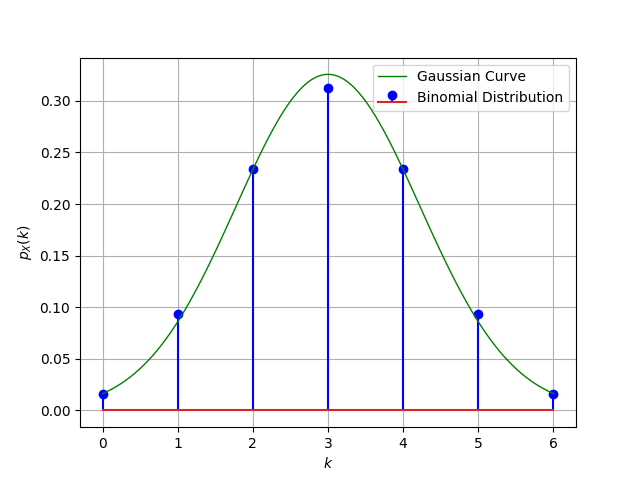
\includegraphics[width=\columnwidth]{figures/PDF_and_PMF.png}
\caption{Binomial Distribution and Gaussian Approximation}
\label{fig:Triangle}
\end{figure}

\end{document}